% !TeX root = thesis_main.tex
% ---------------------------------------------------
% ----- Introduction of the template
% ----- for Bachelor-, Master thesis and class papers
% ---------------------------------------------------
%  Created by C. Müller-Birn on 2012-08-17, CC-BY-SA 3.0.
%  Last upadte: C. Müller-Birn 2015-11-27 
%  Freie Universität Berlin, Institute of Computer Science, Human Centered Computing. 
%
\chapter{Introduction}
\label{chap:introduction}

\section{Topic and context}

In the evergrowing world of software companies, many once startups are now in the situation where they maintain a large software ecosystem and have complcated dependencies of other services or users,
but still want to improve their systems by developing new components and tools.

This poses the challenge of improving the software from aspects like user expeirence, scalability and maintainability while beeing restricted by the ecosystem.
Greenfield development, as it is taught for the majority of books, can't be applied freely without breaking existing features or behaviours.
Thus, applying HCI methods for user research and user experience-focused design might needs to be approached in a diffrent way then during greenfield development.
Also, the common problem of tight deadlines and limited resources allocated by managers tend to lead to premature releases and unstable software.
Instead of developing software to maximize the three HCI factors \textbf{See HCD principles / factors src, anme the tree?} for the actual users, often ideas from individual stakeholders like the executive floor are realized without adding real value.

On the other hand, having an exsisting user base which works with exisiting tools is a great fundament to evaluate what ''real users'' need. So HCI methods applied to them can yield more helpful and focused results. \textbf{rephrase}

Many of the resources or literature about HCI seem to assume a mostly free degree while developing new tools, and also assume a wide user base with diverse demographic features \textbf{is this valid engilsh?}.
\\
\textbf{List literature srces that dont speak about brownfield development?}
\textbf{Find a contra example that does cope with brownfield}
	

\section{Goals of this work}
\begin{itemize}
	\item Was sind die mit dieser Arbeit verfolgten Ziele? Welches Problem soll gelöst werden?
	\item Eine Beschreibung der ersten Ideen, der vorgeschlagene Ansatz und die aktuell erreichten Resultate 
	\item Eine Beschreibung, welchen Beitrag die Arbeit leistet, um das vorgestellte Problem zu lösen
	\item Eine Diskussion, wie die vorgeschlagene Lösung sich von bestehenden unterscheidet, was ist neu oder besser?
\end{itemize}

The goal of this thesis is to implement a new software product, an UI Editor for Apps \& Websites of digital publishing customers,
which is embedded in an existing software ecosystem. During that process, diffrent HCI methods get applied and  

\section{Procedure for the research and implementation}

While writing the software and thesis, I followed the an software design process described in \cite[p. 104]{LearnHCI:2020ys}.
There, the process is divided into a ''Idea'' phase using design thinking, lean ux for first prototypes and then agile development (in my case a relaxed SCRUM version).
Abstractly it looks as following:

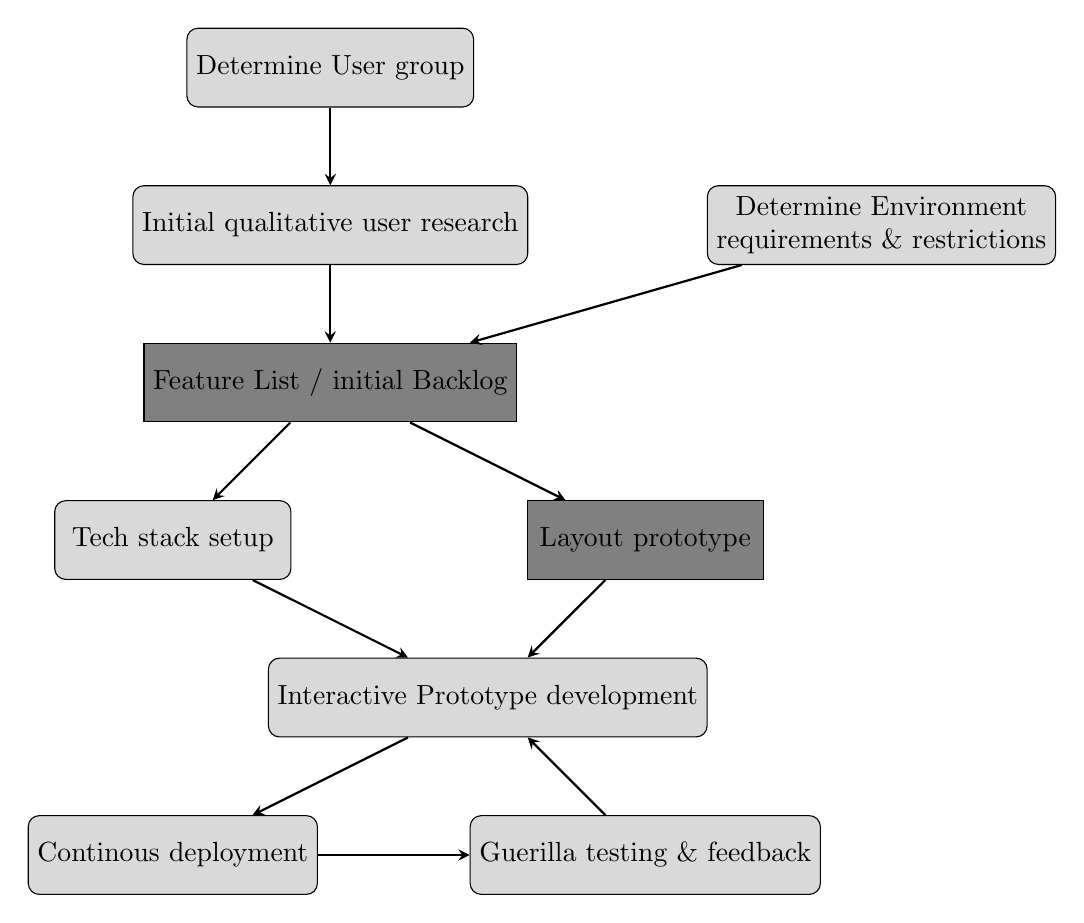
\begin{tikzpicture}[node distance=2cm]
  \tikzstyle{round} = [rectangle, rounded corners, minimum width=3cm, minimum height=1cm,text centered, draw=black, fill=gray!30]
  \tikzstyle{rect} = [rectangle, minimum width=3cm, minimum height=1cm,text centered, draw=black, fill=gray]
  \tikzstyle{arrow} = [thick,->,>=stealth]

  \node (dug) [round] {Determine User group};
  \node (interview1) [round, below of=dug] {Initial qualitative user research};
  \node (denv) [round, right of=interview1, xshift=5cm, align=center] {Determine Environment\\requirements \& restrictions};
  \draw [arrow] (dug) -- (interview1);
  \node (bl) [rect, below of=interview1] {Feature List / initial Backlog};
  \draw [arrow] (denv) -- (bl);
  \draw [arrow] (interview1) -- (bl);
  \node (tech1) [round, below of=bl, xshift=-2cm] {Tech stack setup};
  \node (layout) [rect, right of=tech1, xshift=4cm] {Layout prototype};
  \draw [arrow] (bl) -- (tech1);
  \draw [arrow] (bl) -- (layout);
  \node (proto) [round, below of=tech1, xshift=4cm] {Interactive Prototype development};
  \draw [arrow] (tech1) -- (proto);
  \draw [arrow] (layout) -- (proto);
  \node (deploy) [round, below of=proto, xshift=-4cm] {Continous deployment};
  \draw [arrow] (proto) -- (deploy);
  \node (feedback) [round, right of=deploy, xshift=4cm] {Guerilla testing \& feedback};
  \draw [arrow] (deploy) -- (feedback);
  \draw [arrow] (feedback) -- (proto);
\end{tikzpicture}
  


% \section{Aufbau der Arbeit}
% \begin{itemize}
% 	\item Welche Schritte werden durchlaufen, um die Ziele zu erreichen?
% 	\item An dieser Stelle ist beispielsweise eine Grafik hilfreich, um den Aufbau der Arbeit und welche Ergebnisse/Erkenntnisse wo genutzt werden, zu visualisieren. 
% 	\item Ebenfalls sollten noch Anmerkungen zur Gestaltung der Arbeit gegeben werden, vor allem, da in vielen deutschen Arbeiten englische Fachbegriffe verwendet werden. Ein solcher Text könnte folgendermaßen lauten: 
% 		\begin{itemize}
% 			\item ``Abschließend sind hier noch eine Anmerkungen zur Gestaltung der vorliegenden Arbeit. Für die im Folgenden verwendeten personenbezogene Ausdrücke wurde, um die Lesbarkeit der Arbeit zu erhöhen, die männliche Schreibweise gewählt. Des Weiteren werden eine Reihe von englischen Bezeichnungen verwendet, um einerseits dem interessierten Leser das Studium der häufig vorliegenden englischen Originalliteratur zu erleichtern oder andererseits bestehende Fachbegriffe nicht durch die Übersetzung zu verfälschen. Diese Begriffe sind vom herkömmlichen Text in kursiver Schrift unterschieden.''
% 		\end{itemize}
% \end{itemize}

% \begin{figure}[!ht]
% 	% Mit [!h] wird die Position der Grafik bestimmt. So bedeutet h=here und mit dem "!" (Ausrufezeichen) wird dieser Befehl verstärkt. Weitere Möglichkeiten sind : t=top und b=bottom. Zumeist wird angegeben, in welcher Reihenfolge LaTeX versuchen soll das Bild einzufügen, z.B. [!htb].
% 	\centering
% 		\includegraphics[width=0.95\textwidth]{pics/structure.pdf}
% 	\caption[Beispiel einer möglichen Darstellung zum Aufbau der Arbeit]{Beispiel einer möglichen Darstellung zum Aufbau der Arbeit (vgl. Beschreibung Abschnitt  \ref{chap:chapters}).} 
% 	% Mit Hilfe von caption wird die Bildunterschrift erzeugt. Der Text in geschweiften Klammern erscheint im Text, während der Text in eckigen Klammern sich dann empfiehlt, wenn die Beschreibung besonders lang ist, denn diese wird dann im Bildverzeichnis verwendet. Diese Kurzbeschreibung kann auch weggelassen werden. 
% 	\label{fig:structurethesis}
% \end{figure}